\documentclass[]{article}
\usepackage{lmodern}
\usepackage{amssymb,amsmath}
\usepackage{ifxetex,ifluatex}
\usepackage{fixltx2e} % provides \textsubscript
\ifnum 0\ifxetex 1\fi\ifluatex 1\fi=0 % if pdftex
  \usepackage[T1]{fontenc}
  \usepackage[utf8]{inputenc}
\else % if luatex or xelatex
  \ifxetex
    \usepackage{mathspec}
  \else
    \usepackage{fontspec}
  \fi
  \defaultfontfeatures{Ligatures=TeX,Scale=MatchLowercase}
\fi
% use upquote if available, for straight quotes in verbatim environments
\IfFileExists{upquote.sty}{\usepackage{upquote}}{}
% use microtype if available
\IfFileExists{microtype.sty}{%
\usepackage{microtype}
\UseMicrotypeSet[protrusion]{basicmath} % disable protrusion for tt fonts
}{}
\usepackage[margin=1in]{geometry}
\usepackage{hyperref}
\hypersetup{unicode=true,
            pdftitle={Reproducible Research: Peer Assessment 1},
            pdfborder={0 0 0},
            breaklinks=true}
\urlstyle{same}  % don't use monospace font for urls
\usepackage{color}
\usepackage{fancyvrb}
\newcommand{\VerbBar}{|}
\newcommand{\VERB}{\Verb[commandchars=\\\{\}]}
\DefineVerbatimEnvironment{Highlighting}{Verbatim}{commandchars=\\\{\}}
% Add ',fontsize=\small' for more characters per line
\usepackage{framed}
\definecolor{shadecolor}{RGB}{248,248,248}
\newenvironment{Shaded}{\begin{snugshade}}{\end{snugshade}}
\newcommand{\KeywordTok}[1]{\textcolor[rgb]{0.13,0.29,0.53}{\textbf{#1}}}
\newcommand{\DataTypeTok}[1]{\textcolor[rgb]{0.13,0.29,0.53}{#1}}
\newcommand{\DecValTok}[1]{\textcolor[rgb]{0.00,0.00,0.81}{#1}}
\newcommand{\BaseNTok}[1]{\textcolor[rgb]{0.00,0.00,0.81}{#1}}
\newcommand{\FloatTok}[1]{\textcolor[rgb]{0.00,0.00,0.81}{#1}}
\newcommand{\ConstantTok}[1]{\textcolor[rgb]{0.00,0.00,0.00}{#1}}
\newcommand{\CharTok}[1]{\textcolor[rgb]{0.31,0.60,0.02}{#1}}
\newcommand{\SpecialCharTok}[1]{\textcolor[rgb]{0.00,0.00,0.00}{#1}}
\newcommand{\StringTok}[1]{\textcolor[rgb]{0.31,0.60,0.02}{#1}}
\newcommand{\VerbatimStringTok}[1]{\textcolor[rgb]{0.31,0.60,0.02}{#1}}
\newcommand{\SpecialStringTok}[1]{\textcolor[rgb]{0.31,0.60,0.02}{#1}}
\newcommand{\ImportTok}[1]{#1}
\newcommand{\CommentTok}[1]{\textcolor[rgb]{0.56,0.35,0.01}{\textit{#1}}}
\newcommand{\DocumentationTok}[1]{\textcolor[rgb]{0.56,0.35,0.01}{\textbf{\textit{#1}}}}
\newcommand{\AnnotationTok}[1]{\textcolor[rgb]{0.56,0.35,0.01}{\textbf{\textit{#1}}}}
\newcommand{\CommentVarTok}[1]{\textcolor[rgb]{0.56,0.35,0.01}{\textbf{\textit{#1}}}}
\newcommand{\OtherTok}[1]{\textcolor[rgb]{0.56,0.35,0.01}{#1}}
\newcommand{\FunctionTok}[1]{\textcolor[rgb]{0.00,0.00,0.00}{#1}}
\newcommand{\VariableTok}[1]{\textcolor[rgb]{0.00,0.00,0.00}{#1}}
\newcommand{\ControlFlowTok}[1]{\textcolor[rgb]{0.13,0.29,0.53}{\textbf{#1}}}
\newcommand{\OperatorTok}[1]{\textcolor[rgb]{0.81,0.36,0.00}{\textbf{#1}}}
\newcommand{\BuiltInTok}[1]{#1}
\newcommand{\ExtensionTok}[1]{#1}
\newcommand{\PreprocessorTok}[1]{\textcolor[rgb]{0.56,0.35,0.01}{\textit{#1}}}
\newcommand{\AttributeTok}[1]{\textcolor[rgb]{0.77,0.63,0.00}{#1}}
\newcommand{\RegionMarkerTok}[1]{#1}
\newcommand{\InformationTok}[1]{\textcolor[rgb]{0.56,0.35,0.01}{\textbf{\textit{#1}}}}
\newcommand{\WarningTok}[1]{\textcolor[rgb]{0.56,0.35,0.01}{\textbf{\textit{#1}}}}
\newcommand{\AlertTok}[1]{\textcolor[rgb]{0.94,0.16,0.16}{#1}}
\newcommand{\ErrorTok}[1]{\textcolor[rgb]{0.64,0.00,0.00}{\textbf{#1}}}
\newcommand{\NormalTok}[1]{#1}
\usepackage{graphicx,grffile}
\makeatletter
\def\maxwidth{\ifdim\Gin@nat@width>\linewidth\linewidth\else\Gin@nat@width\fi}
\def\maxheight{\ifdim\Gin@nat@height>\textheight\textheight\else\Gin@nat@height\fi}
\makeatother
% Scale images if necessary, so that they will not overflow the page
% margins by default, and it is still possible to overwrite the defaults
% using explicit options in \includegraphics[width, height, ...]{}
\setkeys{Gin}{width=\maxwidth,height=\maxheight,keepaspectratio}
\IfFileExists{parskip.sty}{%
\usepackage{parskip}
}{% else
\setlength{\parindent}{0pt}
\setlength{\parskip}{6pt plus 2pt minus 1pt}
}
\setlength{\emergencystretch}{3em}  % prevent overfull lines
\providecommand{\tightlist}{%
  \setlength{\itemsep}{0pt}\setlength{\parskip}{0pt}}
\setcounter{secnumdepth}{0}
% Redefines (sub)paragraphs to behave more like sections
\ifx\paragraph\undefined\else
\let\oldparagraph\paragraph
\renewcommand{\paragraph}[1]{\oldparagraph{#1}\mbox{}}
\fi
\ifx\subparagraph\undefined\else
\let\oldsubparagraph\subparagraph
\renewcommand{\subparagraph}[1]{\oldsubparagraph{#1}\mbox{}}
\fi

%%% Use protect on footnotes to avoid problems with footnotes in titles
\let\rmarkdownfootnote\footnote%
\def\footnote{\protect\rmarkdownfootnote}

%%% Change title format to be more compact
\usepackage{titling}

% Create subtitle command for use in maketitle
\newcommand{\subtitle}[1]{
  \posttitle{
    \begin{center}\large#1\end{center}
    }
}

\setlength{\droptitle}{-2em}

  \title{Reproducible Research: Peer Assessment 1}
    \pretitle{\vspace{\droptitle}\centering\huge}
  \posttitle{\par}
    \author{}
    \preauthor{}\postauthor{}
    \date{}
    \predate{}\postdate{}
  

\begin{document}
\maketitle

\subsection{Setup}\label{setup}

\begin{Shaded}
\begin{Highlighting}[]
\NormalTok{knitr}\OperatorTok{::}\NormalTok{opts_chunk}\OperatorTok{$}\KeywordTok{set}\NormalTok{(}\DataTypeTok{echo =} \OtherTok{TRUE}\NormalTok{)}
\KeywordTok{library}\NormalTok{(dplyr)}
\end{Highlighting}
\end{Shaded}

\begin{verbatim}
## 
## Attaching package: 'dplyr'
\end{verbatim}

\begin{verbatim}
## The following objects are masked from 'package:stats':
## 
##     filter, lag
\end{verbatim}

\begin{verbatim}
## The following objects are masked from 'package:base':
## 
##     intersect, setdiff, setequal, union
\end{verbatim}

\begin{Shaded}
\begin{Highlighting}[]
\KeywordTok{library}\NormalTok{(tidyr)}
\KeywordTok{library}\NormalTok{(lubridate)}
\end{Highlighting}
\end{Shaded}

\begin{verbatim}
## 
## Attaching package: 'lubridate'
\end{verbatim}

\begin{verbatim}
## The following object is masked from 'package:base':
## 
##     date
\end{verbatim}

\begin{Shaded}
\begin{Highlighting}[]
\KeywordTok{library}\NormalTok{(lattice)}
\end{Highlighting}
\end{Shaded}

\subsection{Loading and preprocessing the
data}\label{loading-and-preprocessing-the-data}

\begin{Shaded}
\begin{Highlighting}[]
\KeywordTok{setwd}\NormalTok{(}\StringTok{"~/Documents/Classes/DataSciCourse/RepData_PeerAssessment1"}\NormalTok{)}
\NormalTok{data <-}\StringTok{ }\KeywordTok{read.csv}\NormalTok{(}\KeywordTok{unz}\NormalTok{(}\StringTok{'activity.zip'}\NormalTok{, }\StringTok{"activity.csv"}\NormalTok{), }\DataTypeTok{colClasses =} \KeywordTok{c}\NormalTok{(}\StringTok{"numeric"}\NormalTok{, }
                                                \StringTok{"character"}\NormalTok{, }\StringTok{"character"}\NormalTok{))}
\NormalTok{data <-}\StringTok{ }\KeywordTok{as_tibble}\NormalTok{(data)}
\NormalTok{data}
\end{Highlighting}
\end{Shaded}

\begin{verbatim}
## # A tibble: 17,568 x 3
##    steps date       interval
##    <dbl> <chr>      <chr>   
##  1    NA 2012-10-01 0       
##  2    NA 2012-10-01 5       
##  3    NA 2012-10-01 10      
##  4    NA 2012-10-01 15      
##  5    NA 2012-10-01 20      
##  6    NA 2012-10-01 25      
##  7    NA 2012-10-01 30      
##  8    NA 2012-10-01 35      
##  9    NA 2012-10-01 40      
## 10    NA 2012-10-01 45      
## # ... with 17,558 more rows
\end{verbatim}

Date was imported as a character. Let's fix that and the intervals. The
intervals are in the following base 60 format: HHMM where H is an hour
digit and M is a minute digit. This makes a linear plot of the interval
data skip large sections of base 10 space. Here are the date
conversions:

\begin{Shaded}
\begin{Highlighting}[]
\CommentTok{# This 'for' loop converts the intervals to raw minutes}
\NormalTok{data <-}\StringTok{ }\NormalTok{data }\OperatorTok\StringTok{ }\KeywordTok{mutate}\NormalTok{(}\DataTypeTok{Minutes =} \OtherTok{NA}\NormalTok{)}
\ControlFlowTok{for}\NormalTok{(i }\ControlFlowTok{in} \DecValTok{1}\OperatorTok{:}\KeywordTok{dim}\NormalTok{(data)[}\DecValTok{1}\NormalTok{]) \{}
        \ControlFlowTok{if}\NormalTok{(}\KeywordTok{nchar}\NormalTok{(data[i, }\DecValTok{3}\NormalTok{]) }\OperatorTok{<=}\StringTok{ }\DecValTok{2}\NormalTok{)\{}
\NormalTok{                data}\OperatorTok{$}\NormalTok{Minutes[i] =}\StringTok{ }\KeywordTok{as.numeric}\NormalTok{(data[i, }\DecValTok{3}\NormalTok{])}
\NormalTok{        \} }\ControlFlowTok{else} \ControlFlowTok{if}\NormalTok{(}\KeywordTok{nchar}\NormalTok{(data[i, }\DecValTok{3}\NormalTok{]) }\OperatorTok{==}\StringTok{ }\DecValTok{3}\NormalTok{)\{}
\NormalTok{                data}\OperatorTok{$}\NormalTok{Minutes[i] =}\StringTok{ }\DecValTok{60}\OperatorTok{*}\KeywordTok{as.numeric}\NormalTok{(}\KeywordTok{substr}\NormalTok{(data[i, }\DecValTok{3}\NormalTok{], }\DecValTok{1}\NormalTok{, }\DecValTok{1}\NormalTok{)) }\OperatorTok{+}\StringTok{ }
\StringTok{                                   }\KeywordTok{as.numeric}\NormalTok{(}\KeywordTok{substr}\NormalTok{(data[i, }\DecValTok{3}\NormalTok{], }\DecValTok{2}\NormalTok{, }\DecValTok{3}\NormalTok{))}
\NormalTok{        \} }\ControlFlowTok{else} \ControlFlowTok{if}\NormalTok{(}\KeywordTok{nchar}\NormalTok{(data[i, }\DecValTok{3}\NormalTok{]) }\OperatorTok{==}\StringTok{ }\DecValTok{4}\NormalTok{)\{}
\NormalTok{                data}\OperatorTok{$}\NormalTok{Minutes[i] =}\StringTok{ }\DecValTok{60}\OperatorTok{*}\KeywordTok{as.numeric}\NormalTok{(}\KeywordTok{substr}\NormalTok{(data[i, }\DecValTok{3}\NormalTok{], }\DecValTok{1}\NormalTok{, }\DecValTok{2}\NormalTok{)) }\OperatorTok{+}\StringTok{ }
\StringTok{                                   }\KeywordTok{as.numeric}\NormalTok{(}\KeywordTok{substr}\NormalTok{(data[i, }\DecValTok{3}\NormalTok{], }\DecValTok{3}\NormalTok{, }\DecValTok{4}\NormalTok{))}
\NormalTok{        \}}
\NormalTok{\}}

\CommentTok{# This 'for' loop will reformat the intervals to be "HH:MM". Some of the }
\CommentTok{#       intervals have only one, two, or three digits and this must be taken}
\CommentTok{#       into account with the 'if' statements.}
\ControlFlowTok{for}\NormalTok{(i }\ControlFlowTok{in} \DecValTok{1}\OperatorTok{:}\KeywordTok{dim}\NormalTok{(data)[}\DecValTok{1}\NormalTok{]) \{}
        \ControlFlowTok{if}\NormalTok{(}\KeywordTok{nchar}\NormalTok{(data[i, }\DecValTok{3}\NormalTok{]) }\OperatorTok{==}\StringTok{ }\DecValTok{1}\NormalTok{)\{}
\NormalTok{                data[i, }\DecValTok{3}\NormalTok{] =}\StringTok{ }\KeywordTok{paste}\NormalTok{(}\StringTok{"00:0"}\NormalTok{, data[i, }\DecValTok{3}\NormalTok{], }\DataTypeTok{sep =} \StringTok{""}\NormalTok{)}
\NormalTok{        \} }\ControlFlowTok{else} \ControlFlowTok{if}\NormalTok{(}\KeywordTok{nchar}\NormalTok{(data[i, }\DecValTok{3}\NormalTok{]) }\OperatorTok{==}\StringTok{ }\DecValTok{2}\NormalTok{)\{}
\NormalTok{                data[i, }\DecValTok{3}\NormalTok{] =}\StringTok{ }\KeywordTok{paste}\NormalTok{(}\StringTok{"00:"}\NormalTok{, data[i, }\DecValTok{3}\NormalTok{], }\DataTypeTok{sep =} \StringTok{""}\NormalTok{)}
\NormalTok{        \} }\ControlFlowTok{else} \ControlFlowTok{if}\NormalTok{(}\KeywordTok{nchar}\NormalTok{(data[i, }\DecValTok{3}\NormalTok{]) }\OperatorTok{==}\StringTok{ }\DecValTok{3}\NormalTok{)\{}
\NormalTok{                data[i, }\DecValTok{3}\NormalTok{] =}\StringTok{ }\KeywordTok{paste}\NormalTok{(}\StringTok{"0"}\NormalTok{, }\KeywordTok{substr}\NormalTok{(data[i, }\DecValTok{3}\NormalTok{], }\DecValTok{1}\NormalTok{, }\DecValTok{1}\NormalTok{), }\StringTok{":"}\NormalTok{, }
                                   \KeywordTok{substr}\NormalTok{(data[i, }\DecValTok{3}\NormalTok{], }\DecValTok{2}\NormalTok{, }\DecValTok{3}\NormalTok{), }\DataTypeTok{sep =} \StringTok{""}\NormalTok{)}
\NormalTok{        \} }\ControlFlowTok{else} \ControlFlowTok{if}\NormalTok{(}\KeywordTok{nchar}\NormalTok{(data[i, }\DecValTok{3}\NormalTok{]) }\OperatorTok{==}\StringTok{ }\DecValTok{4}\NormalTok{)\{}
\NormalTok{                data[i, }\DecValTok{3}\NormalTok{] =}\StringTok{ }\KeywordTok{paste}\NormalTok{(}\KeywordTok{substr}\NormalTok{(data[i, }\DecValTok{3}\NormalTok{], }\DecValTok{1}\NormalTok{, }\DecValTok{2}\NormalTok{), }\StringTok{":"}\NormalTok{, }
                                   \KeywordTok{substr}\NormalTok{(data[i, }\DecValTok{3}\NormalTok{], }\DecValTok{3}\NormalTok{, }\DecValTok{4}\NormalTok{), }\DataTypeTok{sep =} \StringTok{""}\NormalTok{)}
\NormalTok{        \}}
\NormalTok{\}}

\NormalTok{data <-}\StringTok{ }\NormalTok{data }\OperatorTok\StringTok{ }\KeywordTok{mutate}\NormalTok{(}\DataTypeTok{date_time =} \KeywordTok{as.POSIXct}\NormalTok{(}\KeywordTok{paste}\NormalTok{(date, interval), }
                       \DataTypeTok{format =} \StringTok{"%Y-%m-%d %H:%M"}\NormalTok{), }\DataTypeTok{date =} \KeywordTok{ymd}\NormalTok{(date))}

\NormalTok{data}
\end{Highlighting}
\end{Shaded}

\begin{verbatim}
## # A tibble: 17,568 x 5
##    steps date       interval Minutes date_time          
##    <dbl> <date>     <chr>      <dbl> <dttm>             
##  1    NA 2012-10-01 00:00          0 2012-10-01 00:00:00
##  2    NA 2012-10-01 00:05          5 2012-10-01 00:05:00
##  3    NA 2012-10-01 00:10         10 2012-10-01 00:10:00
##  4    NA 2012-10-01 00:15         15 2012-10-01 00:15:00
##  5    NA 2012-10-01 00:20         20 2012-10-01 00:20:00
##  6    NA 2012-10-01 00:25         25 2012-10-01 00:25:00
##  7    NA 2012-10-01 00:30         30 2012-10-01 00:30:00
##  8    NA 2012-10-01 00:35         35 2012-10-01 00:35:00
##  9    NA 2012-10-01 00:40         40 2012-10-01 00:40:00
## 10    NA 2012-10-01 00:45         45 2012-10-01 00:45:00
## # ... with 17,558 more rows
\end{verbatim}

\subsection{What is mean total number of steps taken per
day?}\label{what-is-mean-total-number-of-steps-taken-per-day}

Let's group by day and take some summary statistics.

\begin{Shaded}
\begin{Highlighting}[]
\NormalTok{data <-}\StringTok{ }\KeywordTok{group_by}\NormalTok{(data, date)}
\NormalTok{sum_steps <-}\StringTok{ }\KeywordTok{summarise}\NormalTok{(data, }\DataTypeTok{sum =} \KeywordTok{sum}\NormalTok{(steps, }\DataTypeTok{na.rm =} \OtherTok{TRUE}\NormalTok{))}

\CommentTok{# Storing the mean and median for future calls.}
\NormalTok{avg <-}\StringTok{ }\KeywordTok{mean}\NormalTok{(sum_steps}\OperatorTok{$}\NormalTok{sum)}
\NormalTok{med <-}\StringTok{ }\KeywordTok{median}\NormalTok{(sum_steps}\OperatorTok{$}\NormalTok{sum)}

\CommentTok{# The histogram. 30 breaks looks better than the default.}
\KeywordTok{hist}\NormalTok{(sum_steps}\OperatorTok{$}\NormalTok{sum, }\DataTypeTok{breaks =} \DecValTok{30}\NormalTok{, }\DataTypeTok{main =} \StringTok{'Histogram of Total Steps Taken in 61 Days'}\NormalTok{, }\DataTypeTok{xlab =} \StringTok{'Total Steps Taken'}\NormalTok{)}
\KeywordTok{box}\NormalTok{()}
\end{Highlighting}
\end{Shaded}

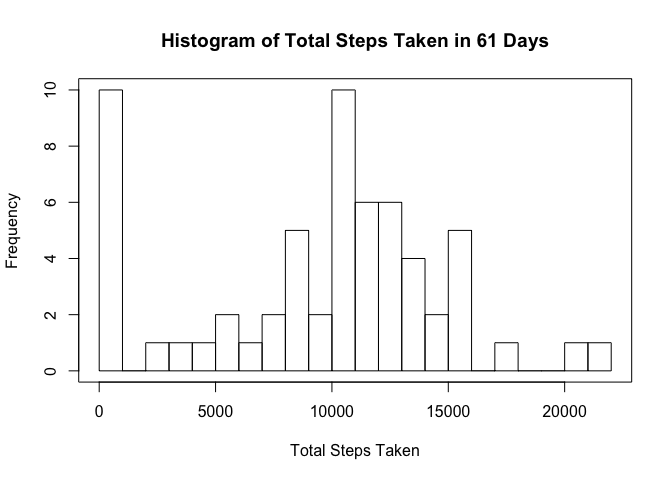
\includegraphics{PA1_template_files/figure-latex/DayGrouping-1.pdf}

The mean number of steps taken each day is 9354.2295082 and the median
is 1.0395\times 10\^{}\{4\}.

\subsection{What is the average daily activity
pattern?}\label{what-is-the-average-daily-activity-pattern}

\begin{Shaded}
\begin{Highlighting}[]
\NormalTok{data <-}\StringTok{ }\KeywordTok{group_by}\NormalTok{(data, Minutes)}
\NormalTok{avg_steps <-}\StringTok{ }\KeywordTok{summarize}\NormalTok{(data, }\DataTypeTok{mean =}  \KeywordTok{mean}\NormalTok{(steps, }\DataTypeTok{na.rm =} \OtherTok{TRUE}\NormalTok{))}
\NormalTok{maximum <-}\StringTok{ }\KeywordTok{max}\NormalTok{(avg_steps}\OperatorTok{$}\NormalTok{mean)}
\NormalTok{max_interval <-}\StringTok{ }\NormalTok{avg_steps[avg_steps}\OperatorTok{$}\NormalTok{mean }\OperatorTok{==}\StringTok{ }\NormalTok{maximum, }\DecValTok{1}\NormalTok{]}

\KeywordTok{plot}\NormalTok{(avg_steps}\OperatorTok{$}\NormalTok{Minutes}\OperatorTok{/}\DecValTok{60}\NormalTok{, avg_steps}\OperatorTok{$}\NormalTok{mean, }\DataTypeTok{type =} \StringTok{'l'}\NormalTok{, }\DataTypeTok{lwd =} \DecValTok{2}\NormalTok{, }
     \DataTypeTok{xlab =} \StringTok{'Hours of the day'}\NormalTok{, }\DataTypeTok{ylab =} \StringTok{'Average number of steps'}\NormalTok{, }
     \DataTypeTok{main =} \StringTok{'Average steps across 61 days}\CharTok{\textbackslash{}n}\StringTok{and measured in 5 minute intervals'}\NormalTok{)}
\end{Highlighting}
\end{Shaded}

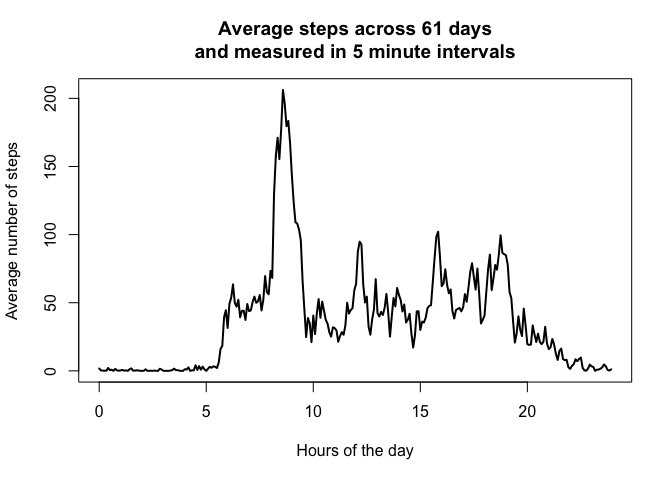
\includegraphics{PA1_template_files/figure-latex/unnamed-chunk-1-1.pdf}

The maximum number of steps in any five minute interval was 206.1698113
steps which started at 8 hours 35 minutes.

\subsection{Imputing missing values}\label{imputing-missing-values}

\begin{Shaded}
\begin{Highlighting}[]
\CommentTok{# Filter for rows with NA steps and get the number of rows.}
\NormalTok{missing <-}\StringTok{ }\KeywordTok{round}\NormalTok{(}\KeywordTok{dim}\NormalTok{(}
        \KeywordTok{filter}\NormalTok{(data, }\KeywordTok{is.na}\NormalTok{(steps))}
\NormalTok{)[}\DecValTok{1}\NormalTok{], }\DecValTok{3}\NormalTok{)}

\CommentTok{# Replace missing values with the average for that interval}
\NormalTok{filled_data <-}\StringTok{ }\NormalTok{data}
\ControlFlowTok{for}\NormalTok{(i }\ControlFlowTok{in} \DecValTok{1}\OperatorTok{:}\KeywordTok{dim}\NormalTok{(data)[}\DecValTok{1}\NormalTok{])\{}
        \ControlFlowTok{if}\NormalTok{(}\KeywordTok{is.na}\NormalTok{(data[i, }\DecValTok{1}\NormalTok{]))\{}
\NormalTok{                filled_data[i,}\DecValTok{1}\NormalTok{] <-}\StringTok{ }
\StringTok{                }\NormalTok{avg_steps[avg_steps}\OperatorTok{$}\NormalTok{Minutes}\OperatorTok{==}\NormalTok{data}\OperatorTok{$}\NormalTok{Minutes[i], }\StringTok{'mean'}\NormalTok{]}
\NormalTok{        \}}
\NormalTok{\}}


\NormalTok{filled_sum_steps <-}\StringTok{ }\NormalTok{filled_data }\OperatorTok\StringTok{ }
\StringTok{        }\KeywordTok{group_by}\NormalTok{(date) }\OperatorTok
\StringTok{        }\KeywordTok{summarise}\NormalTok{(}\DataTypeTok{sum =} \KeywordTok{sum}\NormalTok{(steps, }\DataTypeTok{na.rm =} \OtherTok{TRUE}\NormalTok{))}

\KeywordTok{par}\NormalTok{(}\DataTypeTok{mfcol =} \KeywordTok{c}\NormalTok{(}\DecValTok{1}\NormalTok{,}\DecValTok{2}\NormalTok{))}
\KeywordTok{hist}\NormalTok{(sum_steps}\OperatorTok{$}\NormalTok{sum, }\DataTypeTok{breaks =} \DecValTok{30}\NormalTok{, }\DataTypeTok{main =} \StringTok{'Raw Histogram of Total}\CharTok{\textbackslash{}n}\StringTok{Steps Taken in 61 Days'}\NormalTok{, }\DataTypeTok{xlab =} \StringTok{'Total Steps Taken}\CharTok{\textbackslash{}n}\StringTok{(Raw Data)'}\NormalTok{)}
\KeywordTok{box}\NormalTok{()}
\KeywordTok{hist}\NormalTok{(filled_sum_steps}\OperatorTok{$}\NormalTok{sum, }\DataTypeTok{breaks =} \DecValTok{30}\NormalTok{, }\DataTypeTok{main =} \StringTok{'Filled Histogram of Total}\CharTok{\textbackslash{}n}\StringTok{Steps Taken in 61 Days'}\NormalTok{, }\DataTypeTok{xlab =} \StringTok{'Total Steps Taken}\CharTok{\textbackslash{}n}\StringTok{(Filled Data)'}\NormalTok{)}
\KeywordTok{box}\NormalTok{()}
\end{Highlighting}
\end{Shaded}

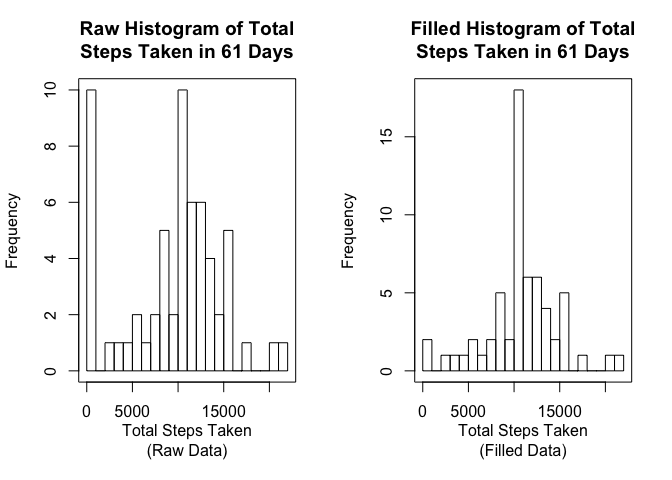
\includegraphics{PA1_template_files/figure-latex/Imputation-1.pdf} There
are 2304 missing values in the `steps' column. They were replaced with
the mean value for the given interval. Eight days that previously had a
total of 0 steps get pushed closer to a total of 10,000 steps. This
causes the mean frequency to become inflated.

\subsection{Are there differences in activity patterns between weekdays
and
weekends?}\label{are-there-differences-in-activity-patterns-between-weekdays-and-weekends}

\begin{Shaded}
\begin{Highlighting}[]
\CommentTok{# First we need to group by Weekday and by Minutes, then take the avg of steps.}
\NormalTok{filled_data}\OperatorTok{$}\NormalTok{Weekdays <-}\StringTok{ }\KeywordTok{factor}\NormalTok{(}\DataTypeTok{x =} \KeywordTok{rep}\NormalTok{(}\OtherTok{NA}\NormalTok{, }\KeywordTok{dim}\NormalTok{(filled_data)[}\DecValTok{1}\NormalTok{]), }
                               \DataTypeTok{levels =} \KeywordTok{c}\NormalTok{(}\StringTok{"Weekday"}\NormalTok{, }\StringTok{"Weekend"}\NormalTok{))}
\NormalTok{MTWRF <-}\StringTok{ }\KeywordTok{c}\NormalTok{(}\StringTok{"Monday"}\NormalTok{, }\StringTok{"Tuesday"}\NormalTok{, }\StringTok{"Wednesday"}\NormalTok{, }\StringTok{"Thursday"}\NormalTok{, }\StringTok{"Friday"}\NormalTok{)}
\ControlFlowTok{for}\NormalTok{(i }\ControlFlowTok{in} \DecValTok{1}\OperatorTok{:}\KeywordTok{dim}\NormalTok{(filled_data)[}\DecValTok{1}\NormalTok{])\{}
        \ControlFlowTok{if}\NormalTok{(}\KeywordTok{weekdays}\NormalTok{(filled_data}\OperatorTok{$}\NormalTok{date[i]) }\OperatorTok\StringTok{ }\NormalTok{MTWRF)\{}
\NormalTok{                filled_data}\OperatorTok{$}\NormalTok{Weekdays[i] <-}\StringTok{ }\KeywordTok{as.factor}\NormalTok{(}\StringTok{"Weekday"}\NormalTok{)}
\NormalTok{        \} }\ControlFlowTok{else}\NormalTok{ \{}
\NormalTok{                filled_data}\OperatorTok{$}\NormalTok{Weekdays[i] <-}\StringTok{ }\KeywordTok{as.factor}\NormalTok{(}\StringTok{"Weekend"}\NormalTok{)}
\NormalTok{        \}}
\NormalTok{\}}

\NormalTok{filled_avg_steps <-}\StringTok{ }\NormalTok{filled_data }\OperatorTok\StringTok{ }
\StringTok{        }\KeywordTok{group_by}\NormalTok{(Weekdays, Minutes) }\OperatorTok
\StringTok{        }\KeywordTok{summarise}\NormalTok{(}\DataTypeTok{Mean =} \KeywordTok{mean}\NormalTok{(steps))}

\KeywordTok{xyplot}\NormalTok{(Mean }\OperatorTok{~}\StringTok{ }\NormalTok{Minutes }\OperatorTok{|}\StringTok{ }\NormalTok{Weekdays, }\DataTypeTok{data =}\NormalTok{ filled_avg_steps, }\DataTypeTok{type =} \StringTok{'l'}\NormalTok{, }
       \DataTypeTok{xlab =} \StringTok{"Interval in minutes"}\NormalTok{, }\DataTypeTok{ylab =} \StringTok{"Mean number of steps"}\NormalTok{, }
       \DataTypeTok{main =} \StringTok{"Average steps in a given interval, by weekday/end"}\NormalTok{, }
       \DataTypeTok{layout =} \KeywordTok{c}\NormalTok{(}\DecValTok{1}\NormalTok{,}\DecValTok{2}\NormalTok{))}
\end{Highlighting}
\end{Shaded}

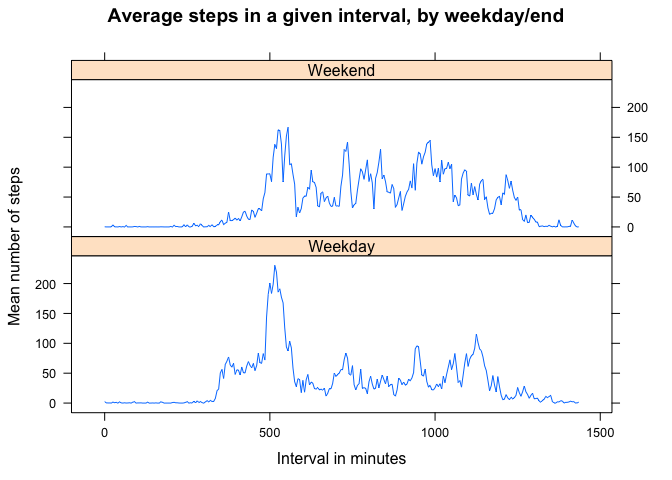
\includegraphics{PA1_template_files/figure-latex/Weekdays-1.pdf}

Weekdays have a larger spike of activity close to 9 am.


\end{document}
